\documentclass[runningheads]{llncs}
\usepackage{graphicx}
\usepackage{float}
\begin{document}
\title{Multisignal digital biosensors for medical applications}
\author{Maren Krafft}
\authorrunning{F. Author et al.}
\institute{Lehrstuhl für technische Informatik, Universität Passau, Germany}
\maketitle        

      
\begin{abstract}
	
Biocomputing has recently gained a place beneath other computing paradigms. Utilizing the natural rules of interaction between biochemical substances, new ways and techniques of solving computing problems have been developed. This review covers the concept of combining so called biosensors, devices that analyse single-input bioprocesses, with the technical possibilities of more complex biochemical logic systems. This combination, utilizing enzymes as the ''machinery'' of biochemical logic systems, aims to create complex analytical biosensors for medical application.



\keywords{Multisignal Biosensors \and Biosensors  \and enzyme-based logic gates \and logic networks \and biomedical applications}
\end{abstract}


\section{Introduction}
%1.Context: what problem is being solved, why relevant or interesting, benefit, possible applications
%2.innovation: described technique completely new or does it improve earlier approcahes? what is improved 
%3.thesolution: how does the presented technique work, core idea of the solution

\subsection{Context}
s
	In the medical field biosensors (analytic devices to convert a biochemical response into an electric signal) are an essential tool for the monitoring and detection of a wide range of medical conditions. The currently available sensors work as single-input devices, that can analyse only one specific substance. New concepts aim to create simple devices, that can analyse multiple inputs and transform those into a single output signal. This change allows for more possible applications.\\
	
	Once realized, those biosensors could revolutionize a great number medical treatments and therapies. Through the analysis of multiple inputs, the sensors could scan specific injuries or diseases. More complex models could even create sense-act-treat devices, that immediately apply the correct treatment after a specific result of the analysis. Especially in medical emergencies, where rapid reactions are of paramount importance, these developments would mark a ground-breaking change. Even personalized medical treatment, which could autonomously adjust the treatment tailored to a patient’s needs, is imaginable.\\
	
	
	In the medical field Biosensors, analytic devices to convert a biological response into a electric signal, are a essential tool for monitoring and detection of a wide range of medical conditions from Diabetes to .....
	While common biosensing devices are limited to a single input, the novelty of Biosensors based on enzyme-based logic systems can process muliple biochemical signals. This article concentrates on the concept of the mulisignal processing Biosensors and the resulting challenges.\\
	
	The basic principle of biosensors are two layers: the receptor, that processes the inputs and the transducer, that translates the received signals to a yes/no-output. The main innovation of the new concept is to replace the current one-input receptor with a biochemical system, that allows a re-creatable analysis of multiple inputs, which are then “summed up” into one output. The receptor usually consists of enzymes (research also produced working systems using DNA and RNA), which react with specific substances. As the result of that reaction is reliable by definition, it produces an exploitable substance, that gets transduced into a yes/no signal.
	

	This document is structures as follows. In Section 2 the concept of Biosensors with enzyme-based logic is introduced. Subsection 2.1 describes the principle of enzyme-based gates and Subsection 2.2 networks of logic gates and the combination with transducers. While section 2 only dealy with the concept of Biosensors section 3 concentrates on the designing of multisignal Biosensors for medical applications.
	In section 4 considerations. Section 5 summarize and outlook. 
\section{concept}

The multisignal processing biosensors in this article are based on enzyme-based logic systems, consisting of chemical logic gates mimicking Boolean operations. Like in common biosensors with single inputs the biosensor is composed by several layers. The receptor, that in common biosensors recognices the selected analyte of interest, is replaced by a enzyme logic systems
The transducer converting biological recognition interaction into a type of signal that is oberservable, for example a electrical current.wortähnlichkeit senses physical changes and converts it into an electrical signal

\subsection{Enzyme-based logic gates and networks}
	
	\subsubsection{Logic gate}
	
	In Biocomputing enzyme as logic in combination with chemical inputs resulting in a end product is used to mimick Boolean logic gates such as AND and OR. To digitalize chemical processes two levels of concentrations of chemical reaction materials are considers as input signals. 0 is usually considered as the absence of a enzyme, but it can be altered. 1 equals a  significantly difference to the absence or the as 0 defined concentration.
	Output signal ein vorher bestimmter stoff, falls dieser vorhanden regel 1 falls nicth regel 0.  
	(Katz) \\
	
	Beispiel AND 
	In Fig 1 glucose oxidase and catalase, which are enzymes, operate as the logic gate machinery. The two input signals H2O2 and glucose. When both substrates present the inputs reacted and produces gluconic acid, which results in anoptical absorbance change, that was defined as the ouput signal of the enzyme logic gate. The optical absorbance change just appeared in the presence of both inputs, mimicking the Boolean operation AND. 

	\begin{figure}[H] \centering 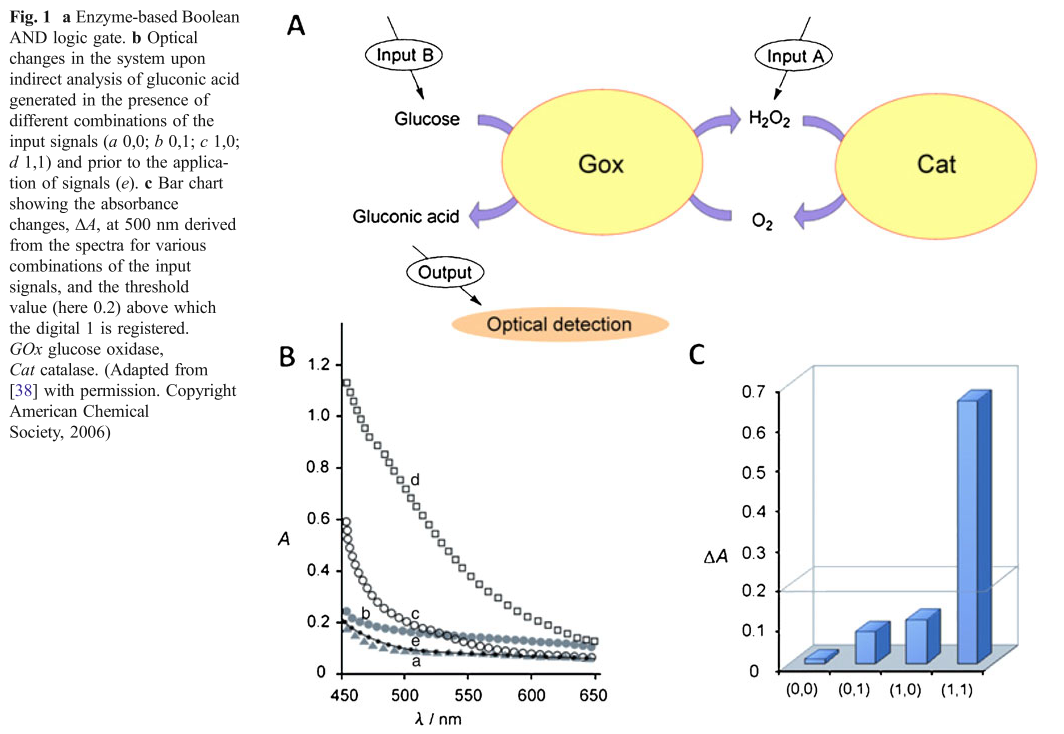
\includegraphics[scale= 0.3]{pics/AND.png} \caption{Network diagramm} \label{img:and} \end{figure}
	
	\subsubsection{networks with electrochemical transduction}
	By assembling these single logic gates, mimicking Boolean operations,it is possible to create small logic networks(e.g. half-adder/ half subtractor)/enzyme logic systems. Transducers missing 
	
	For example, a logic network with three enzymes alchol dehydrogenase, glucose dehydrogenase and glucose oxidase operating as four concatenated logic gates and four different input signals (NADH,  actealdehyde,glucose and oxygen) The cascade of reactions resulted in ph changes. 
	successful case: yielding acid medium,lowering pH from initila ph 6-7 to approcimately 4. The pH scale is defined from 0 (acid solution) to 14 (lye solution).
	%erst kombination von reaktionen
	
	\begin{figure}[H] \centering 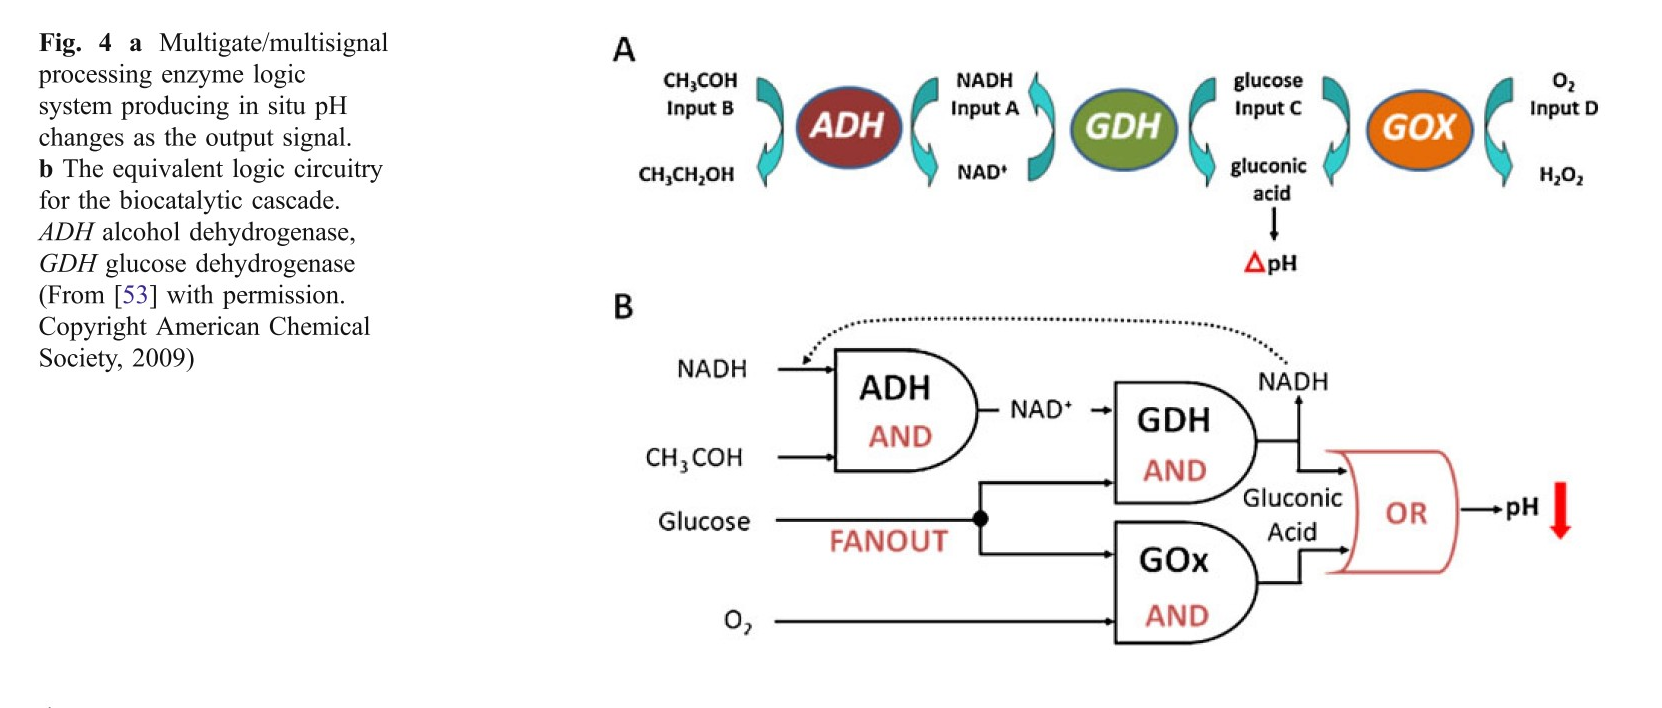
\includegraphics[scale= 0.3]{pics/biocomputing_sensor.png} \caption{Network diagramm} \label{img:grafik-test} \end{figure}
	
	%verbindung mit transducer
	
	The lower pH value resulted in switching to ON of a electrochemical interface that functioned as transducerand and  read out by whatever, volt usw
	While 16 different variants where possible only four combinations resultet in a ON state.

	\begin{figure}[H] \centering 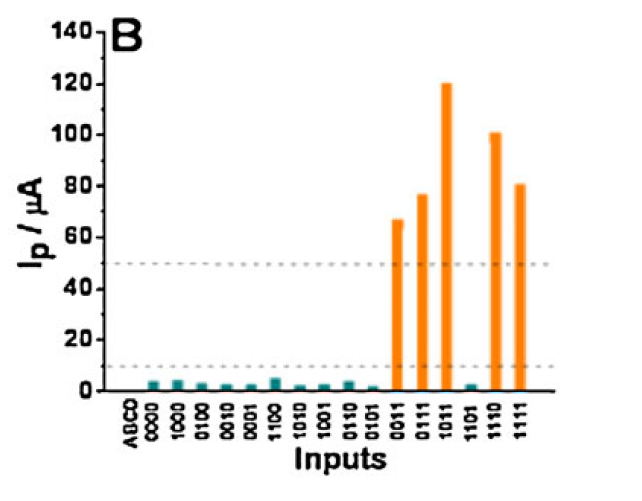
\includegraphics[scale= 0.2]{pics/ph.png} \caption{Network diagramm} \label{img:ph} \end{figure}
	
	
This combination is a example for a multisignal processing enzyme logic system coupled with an electrochemical transduction readout of the output signal (pH change)
\section{designing for biochemical analytic applications}
	\begin{itemize}
		\item design of biosensoric systems with logically processes signals represented by varous biomarkers characteristic for different abnormal physiological conditions
		\item analysis of the chemical output signals generated by biomolecular logic systems is often limited.
		\item Enzyme logic system: multiassemblies to perform simple arithmetic functions
		\item idea: applicatoin of biomolecular logic system for analytical purpose new class of biosensors that accept many input signals and produce binary outputs in form yes/no 
		\item example analyse protein libraties associated with muliple sclerosis(58)
	\end{itemize}

	\begin{itemize}
		\item not just chronic but also ..........
		\item state of the art
		\item feedback loop currently devoted to management of diabetes through integration of an electrochemical glucose sensing element with an insulin-delivery feedback loop for the optimal dose of insulin (69-71)
		\item example analyse protein libraties associated with muliple sclerosis(58)
		
		ENzyme logic system recognizing various injury-related physiological conditions
		\begin{itemize}
			\item types of injuries result in concentrations of chemical substances in the body
			
			\item example: lactate axidase, horeserasish peroxidase and glucose dehydrogenase = designed to process biochemical information related to pathophysiological conditions from brain injury
			\item markers: glucose(hemorrhagic shock),lactate(rhagic shock or traumic brain injury) and norepinephrine(traumatic injury)
			\item logic 0 = normal concentrations
			\item change results into different numbers 1,2,3 - convenient
			\item = biocomputing logic system 
			\item challenge: difference between normal and unnormal minimal => not linear, should be sigmoidal	
		\end{itemize}
	\end{itemize}



\section{considerations}
stabilization and confinement//
optical transduction 
\subsection{surface immobilization of the biocomputing machinery}
	
	
	
	\begin{itemize}
		\item optimal surface confinement of the biocomputing layer
		\item engineering enzyme microenvironment (transducer layer)
		\item contact between biocomputing layer and transducing surface
		\item combine individual logic-gates and maintain high enzymatic stability and reataining individual reagents
		\item leakage of cosubstrate 
		\item no cross-reactions
		\item surface confinement? layer-by layer? more efficient and rational 
		\item level of the surface confined reagents tailored for account of different input concentrations /enzyme activities 
		\item coating: optimized for transport and excluding potential interfernece and protecting the surface
	\end{itemize}

\subsection{optimal transduction of biocomputing signal processes}
	\begin{itemize}
		\item simultaneous measurements of multiple outputs require different transduction strategies (common: fixed potential )
	\end{itemize}
	\begin{itemize}
		\item Requires:interface of biocomputing systems + electronic transducer\\
		Therefore
		\item scalability (increasing nuber of logic gates, assembling into complex networks)
		\item complexity(coupling of gates abd non boolean elements)
		\item composition, preparation and immobilization of the biocomputing surface layer
		\item layer by layer
		\item optimal surface confinement 
		\item careful engineering of the enzyme microenvironment(on transducer surface) for performance
		\item biocomputing layer + transducing layer + combine individual logic-gate elements	
	\end{itemize}



\section{Conclusion}
	good but needs lot of work\\
	sums up bla
	
		Profound impact\\
	
	Through processing automatically several biochemical inputs(physiological information), it can provide a rapid and reliable assessment of overall physiological conditions. This can help a optimal timley therapeutic intervention. They will realize sense/delivery feedback loops by coupling signal processing with chemical actuators to revolutionize patient monitoring and drug delivery. 
	
	In the Biosensors processing multiple biochemical signal, the core idea is to add a biocomputing layer that produces a final output in form of a yes/no response. Kapitel 1.2\\
	
	Chances:
	
	
	
	
	In contrast to recent biosensors, those with a 11111111111 logic promise a higher fidelity, a greater range of processable inputs, more complex applications such as sense-act-treat loops and rapid assessment of the respective substances.(mehr ausformulieren)
	
	
	
	
	\subsection{Biosensors  logic systems}
	Biosensors logically processing multiple biochemical signals\\
	-such procassed information produces a final output yes/no \\
	- boolean logic networks composed of biomolecular systems\\	
	\begin{itemize}
		\item multiple target analytes(inputs) for enzyme gates
		\item high-fidelity compared
		\item closed loop/feedback loops possible (sense/act/treat)
		\item rapid and reliable assessment of overall physiological condition
		\item could initiate optimal timely therapeutic intervention
		\item biosensors + enzyme logic gates
		\item allows direct coupling of signal processing with chemical actuators 
		\item application og biomolecular logic systems for analystic purposes could yield a novel class of biosensors: many input signals and binary outputs
		\item logically processed feedback between drug appl. and physiological conditions can signifacntly imprive drug targeting and efficiency 
		
		\item difficulties: complexity by assembling individual logic gates into complex logic networks (intelligent by molecular logic) (43-34-67)
		\item new approach for the sensor design and operation, interfach biocomputing system and electronic transducers
	\end{itemize}


\begin{thebibliography}{8}
	\bibitem{application}
	Parikha Mehrotra, Biosensors and their applications - A Review (2016)
	
	\bibitem{biosensors}
	Daniel R. Thevenot, Klara Toth, Richard A. Durst, George S. Wilson, Electrochemical biosensors: recommended definitions and classifications In: Biosensors and Bioelectronics 16 (2001) 121- 131
	
	\bibitem{source1}
	Joseph Wang, Evgeny Katz, Digital biosensors with build-in logic for biomedical applications- biosensors based on a biocomputing concept, in: Anal Bioanal Chem(2010) 1591-1603
	
	\bibitem{source2}
	Shengbo Sang, Wendong Zhang and Yuan Zhao, State of the Art in Biosensors, in: State of the Art of Biosensors(2013) 89-110
	
	\bibitem{source3}
	Evgeny Katz, Enzyme-Based Logic Gates and Networks with Outout Signals Analyzed by Various Methods, In: ChemPhysChem 2017, 18 1688-1713
	
\end{thebibliography}
\end{document}
